\chapter{Object Detection}

\label{ch3_OBJ}

%Replace \lipsum with text.
% You may have as many sections as you please. This is just for reference.

Video clips of certain activity class have peculiar set of objects present in it.
If one could find objects present in the video clip, the activity prediction can 
potentially be made more confident. Below sections introduce the object detection
method and its use in this project.

\section{Object Detector}
Object detector based on Discriminatively Trained Deformable Part Models \cite{voc-release4} was used in
the project. It can run on an image at a time. The detectors used in this project are trained on PASCAL 2007 data sets.
There are 20 models corresponding to 20 different objects.
These objects are : aeroplane, bicycle,
bird, boat, bottle, bus, car, cat, chair, cow, dining table, dog, horse,
motorbike, person, potted plant, sheep, sofa, train, tv monitor.
For this project only 10 relevant models were used : bicycle, bottle, bus, car,
chair, diningtable, motorbike, person, sofa, tvmonitor.

\section{Detection in Video}
Above described object detector models work on a single image at a time. To detect objects in video clips, 1 frame per second was extracted from the video clip and all the object detector models were run on the frame. In the data set used in this project, shortest clips is about 3-4 seconds long and longest clips are of the order of a minute. Frame rate is 24 frames per second.

The object detector models give a \index{Bounding Box}bounding box and a confidence (also called \index{Decision Value}decision value) for each detection 
on an absolute scale between $-\infty$ to $\infty$. 
Usually, a positive decision value represents true positive in all the models. 
A negative decision value represent lesser confident detection. 
It might be a true positive or a false positive. 
One can specify a threshold decision value before running object detector model 
so that only the detections at least as confident as the threshold are considered.
Usually, such thresholds are negative to allow detection of lesser confident objects also.

\section{Output of Object Detector}

The visual output of object detector looks as shown in figures \ref{fig:CarDetection} and \ref{fig:PersonDetection}. 
The red boxes are called as bounding boxes.
For each box, a confidence value is also evaluated - also called as decision value.

Table \ref{table:ObjDetection} shows the decision values for sample detections.

\floatstyle{plain}
\restylefloat{figure}
\begin{figure}[here]
\begin{center} 
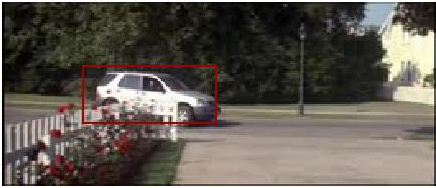
\includegraphics[scale=0.5]{car_detection_1.jpg} 
\caption{ Car detection in a frame. \label{fig:CarDetection}} 
\end{center} 
\end{figure}  

\begin{figure}[here]
\begin{center} 
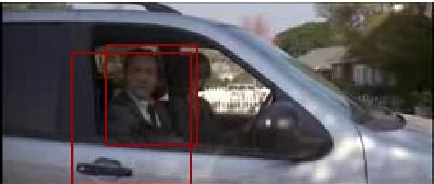
\includegraphics[scale=0.5]{person_detection_151.jpg} 
\caption{ Person detection in a frame. \label{fig:PersonDetection}} 
\end{center} 
\end{figure}  

\begin{table}[t,here]
\centering
\begin{tabular}{|l|c|}
\hline
\multicolumn{2}{|c|}{FRAME1} \\
\hline
 Car            &-0.181786\\
\hline
\multicolumn{1}{|c|}\vdots & \vdots \\
\hline
\multicolumn{1}{|c|}\vdots & \vdots \\
\hline
\multicolumn{2}{|c|}{FRAME151} \\
\hline
Person	&0.579786\\
\hline
Person	&-0.593087\\
\hline
\end{tabular}
\caption{Output of object detector with decision values}
\label{table:ObjDetection}
\end{table}



